% !TEX root = ../thesis.tex

\chapter{Theory and Motivation for Searching for a Dibosonic Resonance}
\label{chap:theory}

\section{Introduction}

The search for new particles has been an ongoing endeavor since the first accelerators came online in the mid-20th century.

% More history here

Today, the Standard Model remains as the dominant theory describing three of the four known forces, with gravity excluded due to its inability to be renormalized when approached as a quantum field theory.
The theory itself stands as one of the most well-tested models of physics in history, and all elementary particles predicted by the theory have been found, with the Higgs completing the family after being discovered in the summer of 2012.
However, despite the success of this theory, many fundamental questions of physics still remain unanswered.
As previously mentioned, the theory does not include gravity, as it only accounts for the electromagnetic, strong, and weak nuclear forces.
It also does not account for the existence of Dark Matter or Dark Energy, and there are long-standing issues that the theory currently is incapable of addressing, such as the hierarchy problem.
The theory is therefore regarded as incomplete, and efforts to find physics beyond the Standard Model are ongoing.

In this chapter, we briefly explore the main aspects of the Standard Model in section~\ref{sec:SM}, looking at its mathematical foundations and the fundamental particles that it describes.
Later, in section~\ref{sec:VBF}, we describe the theoretical background relevant to the search for a new fundamental particle beyond the Standard Model that this thesis presents.

\section{The Standard Model of Particle Physics}
\label{sec:SM}

The Standard Model is the prevailing theory in particle physics that classifies all known elementary particles, and describes how the interact with each other via the electromagnetic, weak, and strong forces.
The theory came about during the 1960's in order to explain observations made during early collision experiments\footnotemark.

\footnotetext{While the theory itself was developed in the 1960's, the term ``Standard Model'' was coined by Pais and Treiman in 1975~\cite{CaoFieldTheory}.} % Citation needed

\begin{figure}[htbp]
  \centering
  % !TEX root = ../../thesis.tex

\begin{tikzpicture}
  % Quarks
  \draw pic at (0,0) {particle={green!20}{$u$}{up}{$2.16$ MeV/$c^2$}{$2/3$}{$1/2$}};
  \draw pic at (0,-2.2) {particle={green!20}{$d$}{down}{$4.67$ MeV/$c^2$}{$-1/3$}{$1/2$}};
  \draw pic at (2.2,0) {particle={green!20}{$c$}{charm}{$1.27$ GeV/$c^2$}{$2/3$}{$1/2$}};
  \draw pic at (2.2,-2.2) {particle={green!20}{$s$}{strange}{$93$ MeV/$c^2$}{$-1/3$}{$1/2$}};
  \draw pic at (4.4,0) {particle={green!20}{$t$}{top}{$172.76$ GeV/$c^2$}{$2/3$}{$1/2$}};
  \draw pic at (4.4,-2.2) {particle={green!20}{$b$}{bottom}{$4.18$ MeV/$c^2$}{$-1/3$}{$1/2$}};

  % Leptons
  \draw pic at (0,-4.4) {particle={red!20}{$e$}{electron}{$511$ keV/$c^2$}{$-1$}{$1/2$}};
  \draw pic at (0,-6.6) {particle={red!20}{$\nu_e$}{$e$ neutrino}{$<1.1$ eV/$c^2$}{$0$}{$1/2$}};
  \draw pic at (2.2,-4.4) {particle={red!20}{$\mu$}{muon}{$105.66$ MeV/$c^2$}{$-1$}{$1/2$}};
  \draw pic at (2.2,-6.6) {particle={red!20}{$\nu_\mu$}{$\mu$ neutrino}{$<0.19$ eV/$c^2$}{$0$}{$1/2$}};
  \draw pic at (4.4,-4.4) {particle={red!20}{$\tau$}{tau}{$1.7769$ GeV/$c^2$}{$-1$}{$1/2$}};
  \draw pic at (4.4,-6.6) {particle={red!20}{$\nu_\tau$}{$\tau$ neutrino}{$<18.2$ MeV/$c^2$}{$0$}{$1/2$}};

  % Gauge Bosons
  \draw pic at (6.6,0) {particle={blue!20}{$g$}{gluon}{$0$}{$0$}{$1$}};
  \draw pic at (6.6,-2.2) {particle={blue!20}{$\gamma$}{photon}{$0$}{$0$}{$1$}};
  \draw pic at (6.6,-4.4) {particle={blue!20}{$Z$}{$Z$ boson}{$91.1876$ GeV/$c^2$}{$0$}{$1$}};
  \draw pic at (6.6,-6.6) {particle={blue!20}{$W$}{$W$ boson}{$80.379$ GeV/$c^2$}{$\pm1$}{$1$}};

  % Scalar Bosons
  \draw pic at (8.8,0) {particle={orange!20}{$H$}{higgs}{$124.97$ GeV/$c^2$}{0}{0}};

  % Labels
  \node at (-1,0.8) [anchor=mid east,scale=0.5] {mass};
  \node at (-1,0.5) [anchor=mid east,scale=0.5] {charge};
  \node at (-1,0.2) [anchor=mid east,scale=0.5] {spin};
  \coordinate (d) at (0,-2.2);
  \coordinate (nu) at (0,-6.6);
  \coordinate (w) at (6.6,-6.6);
  \coordinate (h) at (8.8,0);
  \coordinate (u) at (0,0);
  \coordinate (c) at (2.2,0);
  \coordinate (t) at (4.4,0);
  \node at ($(d)+(-1.35,-1)$) [rotate=90,anchor=mid west,text=green!100] {quarks};
  \node at ($(nu)+(-1.35,-1)$) [rotate=90,anchor=mid west,text=red!100] {leptons};
  \node at ($(w)+(1.35,-1)$) [rotate=90,anchor=mid west,text=blue!100] {gauge bosons};
  \node at ($(h)+(1.35,1)$) [rotate=90,anchor=mid east,text=orange!100] {scalar bosons};
  \node at ($(u)+(0,1.35)$) {I};
  \node at ($(c)+(0,1.35)$) {II};
  \node at ($(t)+(0,1.35)$) {III};
\end{tikzpicture}

  \caption{Table of all standard model particles grouped by generation and type, labeled with mass, charge, and spin~\cite{PhysRevD.98.030001}. Particle types are colored green for quarks, red for leptons, blue for gauge bosons, and yellow for the Higgs.}
  \label{fig:standardModel}
\end{figure}

\section{Search for a Heavy Diboson Resonance and Vector Boson Fusion Production Method}
\label{sec:VBF}

\begin{figure}[htbp]
  \centering
  % !TEX root = ../../thesis.tex
\begin{tikzpicture}
  \begin{feynman}
    % Vertices
    \coordinate (q1) at (-1.5,1.25);
    \coordinate (q2) at (0,1);
    \coordinate (q3) at ($(q2)+(11.5:4.75)$);
    \coordinate (q4) at (-1.5,-1.25);
    \coordinate (q5) at (0,-1);
    \coordinate (q6) at ($(q5)+(-11.5:4.75)$);
    \coordinate (v1) at (1,0);
    \coordinate (x1) at (2.25,0);
    \coordinate (v2) at (3.5,0.75);
    \coordinate (v3) at (3.5,-0.75);
    \coordinate (q7) at ($(v2)+(15:1.25)$);
    \coordinate (q8) at ($(v2)+(-15:1.25)$);
    \coordinate (l1) at ($(v3)+(15:1.25)$);
    \coordinate (l2) at ($(v3)+(-15:1.25)$);

    \coordinate (q9) at ($(q1)+(8.5,0)$);
    \coordinate (q10) at ($(q2)+(8.5,0)$);
    \coordinate (q11) at ($(q3)+(8.5,0)$);
    \coordinate (q12) at ($(q4)+(8.5,0)$);
    \coordinate (q13) at ($(q5)+(8.5,0)$);
    \coordinate (q14) at ($(q6)+(8.5,0)$);
    \coordinate (v4) at ($(v1)+(8.5,0)$);
    \coordinate (x2) at ($(x1)+(8.5,0)$);
    \coordinate (v5) at ($(v2)+(8.5,0)$);
    \coordinate (v6) at ($(v3)+(8.5,0)$);
    \coordinate (q15) at ($(q7)+(8.5,0)$);
    \coordinate (q16) at ($(q8)+(8.5,0)$);
    \coordinate (l3) at ($(l1)+(8.5,0)$);
    \coordinate (l4) at ($(l2)+(8.5,0)$);

    % Lines
    \draw[fermion] (q1) -- (q2);
    \draw[fermion] (q2) -- (q3);
    \draw[fermion] (q4) -- (q5);
    \draw[fermion] (q5) -- (q6);
    \draw[boson] (q2) -- (v1) node[pos=0.65,xshift=-0.5cm] {$Z$};
    \draw[boson] (q5) -- (v1) node[pos=0.65,xshift=-0.5cm] {$Z$};
    \draw[boson] ($(v1)+(0,-0.025)$) -- ($(x1)+(0,-0.025)$);
    \draw[boson] ($(v1)+(0,0.025)$) -- ($(x1)+(0,0.025)$) node[pos=0.5,above] {$X$};
    \draw[boson] (x1) -- (v2) node[pos=0.9,xshift=-0.5cm] {$W$};
    \draw[boson] (x1) -- (v3) node[pos=0.9,xshift=-0.5cm] {$W$};
    \draw[fermion] (v2) -- (q7);
    \draw[fermion] (q8) -- (v2);
    \draw[fermion] (v3) -- (l1);
    \draw[fermion] (l2) -- (v3);

    \draw[fermion] (q9) -- (q10);
    \draw[fermion] (q10) -- (q11);
    \draw[fermion] (q12) -- (q13);
    \draw[fermion] (q13) -- (q14);
    \draw[boson] (q10) -- (v4) node[pos=0.65,xshift=-0.5cm] {$W$};
    \draw[boson] (q13) -- (v4) node[pos=0.65,xshift=-0.5cm] {$Z$};
    \draw[boson] (v4) -- (x2) node[pos=0.5,above] {$X$};
    \draw[scalar] (x2) -- (v5) node[pos=0.9,xshift=-0.5cm] {$H$};
    \draw[boson] (x2) -- (v6) node[pos=0.9,xshift=-0.5cm] {$W$};
    \draw[fermion] (v5) -- (q15);
    \draw[fermion] (q16) -- (v5);
    \draw[fermion] (v6) -- (l3);
    \draw[fermion] (l4) -- (v6);

    % Blobs
    \fill[white] (v1) circle (0.2);
    \fill[white] (x1) circle (0.2);
    \draw[pattern=north west lines] (v1) circle (0.2);
    \draw[pattern=north west lines] (x1) circle (0.2);

    \fill[white] (v4) circle (0.2);
    \fill[white] (x2) circle (0.2);
    \draw[pattern=north west lines] (v4) circle (0.2);
    \draw[pattern=north west lines] (x2) circle (0.2);

    % Labels
    \node[anchor=mid,left] at (q1) {$q''$};
    \node[anchor=mid,left] at (q4) {$q'''$};
    \node[anchor=mid,right] at (q3) {$q''$};
    \node[anchor=mid,right] at (q6) {$q'''$};
    \node[anchor=mid,right] at (q7) {$q$};
    \node[anchor=mid,right] at (q8) {$\bar{q}'$};
    \node[anchor=mid,right] at (l1) {$\ell$};
    \node[anchor=mid,right] at (l2) {$\nu$};

    \node[anchor=mid,left] at (q9) {$q'$};
    \node[anchor=mid,left] at (q12) {$q'''$};
    \node[anchor=mid,right] at (q11) {$q''$};
    \node[anchor=mid,right] at (q14) {$q'''$};
    \node[anchor=mid,right] at (q15) {$b$};
    \node[anchor=mid,right] at (q16) {$\bar{b}$};
    \node[anchor=mid,right] at (l3) {$\ell$};
    \node[anchor=mid,right] at (l4) {$\nu$};
  \end{feynman}
\end{tikzpicture}

  \caption{Feynman diagram for the production of a generic resonance $X$ via vector boson fusion and decaying to the final state $\ell\nu q\bar{q}'$, with additional forward-facing jets due to the VBF production process.}
  \label{fig:vbfFeynman}
\end{figure}

\begin{figure}[htbp]
  \centering
  % !TEX root = ../../thesis.tex

\begin{tikzpicture}
  % Axis
  \draw[->] (-6,0) -- (6,0) node[right] {$z$};

  % Leptons
  \draw[->,thick] (0,0) -- (105:3) node[left] {$\ell$};
  \draw[->,thick] (0,0) -- (75:3) node[right] {$\nu$};

  % Main jet
  \draw[rotate around={180:(0,0)},dotted,thick] (0,2) ellipse (1.3 and 0.4);
  \draw[rotate around={180:(0,0)},dotted,thick] (0,0) -- (56.427:2.3);
  \draw[rotate around={180:(0,0)},dotted,thick] (0,0) -- (123.573:2.3);

  % Sub jets
  \draw[rotate around={180:(0,0)},dotted,thick] (0.5,2) ellipse (0.4 and 0.1);
  \draw[rotate around={180:(0,0)},dotted,thick] (0,0) -- (65.715:2.18);
  \draw[rotate around={180:(0,0)},dotted,thick] (0,0) -- (87.135:2);
  \draw[rotate around={180:(0,0)},dotted,thick] (-0.5,2) ellipse (0.4 and 0.1);
  \draw[rotate around={180:(0,0)},dotted,thick] (0,0) -- (92.865:2);
  \draw[rotate around={180:(0,0)},dotted,thick] (0,0) -- (114.285:2.18);

  % VBF Jets
  \draw[rotate around={80:(0,0)},dotted,thick] (0,4) ellipse (0.5 and 0.1);
  \draw[rotate around={80:(0,0)},dotted,thick] (0,0) -- (82.875:4.03);
  \draw[rotate around={80:(0,0)},dotted,thick] (0,0) -- (97.125:4.03);
  \draw[rotate around={260:(0,0)},dotted,thick] (0,4) ellipse (0.5 and 0.1);
  \draw[rotate around={260:(0,0)},dotted,thick] (0,0) -- (82.875:4.03);
  \draw[rotate around={260:(0,0)},dotted,thick] (0,0) -- (97.125:4.03);

  % Labels
  \node[anchor=mid] at (257.5:2.75) {$q$};
  \node[anchor=mid] at (282.5:2.75) {$\bar{q}^{(\prime)}$};
  \node[anchor=mid] at (170:4.5) {$q^{(\prime)}$};
  \node[anchor=mid] at (350:4.5) {$q^{(\prime)}$};

\end{tikzpicture}

  \caption{Illustration of event topology for VBF collision events in the CMS detector. The semi-leptonic final state produces a $W$ boson that decays via $W\to\ell\nu$ and produces the lepton-neutrino pair. Opposite to that is a single massive jet with two-pronged substructure that is produced via $V\to q\bar{q}^{(\prime)}$. Finally, the VBF production process results in two forward facing jets, each labeled by $q^{(\prime)}$. Selection cuts for the analysis are made in order to search for events with such topology.}
  \label{fig:eventTop}
\end{figure}

\begin{figure}[htbp]
  \centering
  % !TEX root = ../../thesis.tex

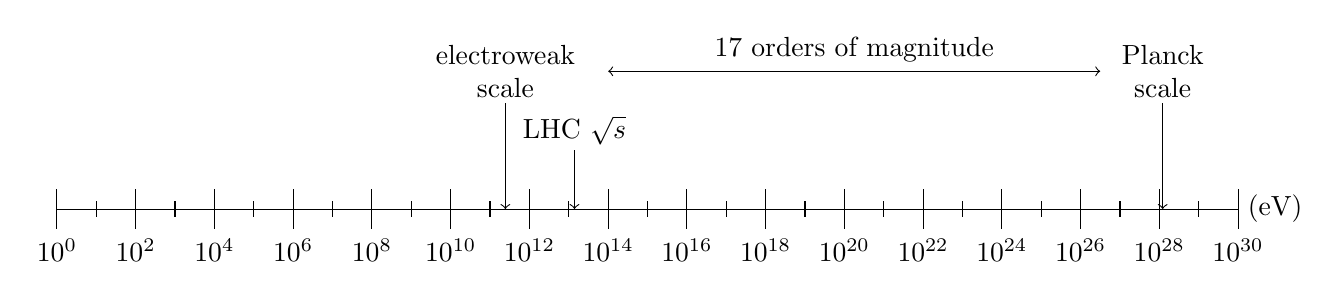
\begin{tikzpicture}
  % Axis
  \draw (0,0) -- (15,0) node[right] {(eV)};
  \draw (0,-0.25) -- (0,0.25);
  \node[below] at (0,-0.25) {$10^0$};

  \foreach \i in {1,...,15}
  {
    % Ticks
    \pgfmathsetmacro{\y}{\i-0.5}
    \draw (\i,-0.25) -- (\i,0.25);
    \draw (\y,-0.1) -- (\y,0.1);

    % Numerical labels
    \pgfmathtruncatemacro{\x}{\i*2}
    \node[below] at (\i,-0.25) {$10^{\x}$};
  }

  % Labels
  \draw[->] (5.695,1.75) node[fill=white,inner sep=2pt,align=center] {electroweak\\scale} -- (5.695,0);
  \draw[->] (6.573,1) node[fill=white,inner sep=2pt] {LHC $\sqrt{s}$} -- (6.573,0);
  \draw[->] (14.043,1.75) node[fill=white,inner sep=2pt,align=center] {Planck\\scale} -- (14.043,0);
  \draw[<->] (7,1.75) -- (13.25,1.75) node[pos=0.5,above] {17 orders of magnitude};
\end{tikzpicture}

  \caption{Comparison between the electroweak scale, LHC center of mass energy $\sqrt{s}$, and Planck scale in eV.}
  \label{fig:hierarchy}
\end{figure}

\begin{figure}[htbp]
  \centering
  % !TEX root = ../../thesis.tex

\begin{tikzpicture}
  \begin{feynman}
    % Vertices
    \coordinate (q1) at (135:2.25);
    \coordinate (q2) at (0,0);
    \coordinate (q3) at (225:2.25);
    \coordinate (l1) at ($(q3)+(5,0)$);
    \coordinate (l2) at ($(l1)+(-25:-1.5)$);
    \coordinate (l3) at ($(l2)+(25:1.5)$);
    \coordinate (g1) at (135:0.5625);
    \coordinate (q4) at ($(q1)+(5,0)$);
    \coordinate (q5) at ($(q4)+(25:-1.5)$);
    \coordinate (q6) at ($(q5)+(-25:1.5)$);

    \coordinate (g2) at ($(7,0)+(135:1.5)$);
    \coordinate (g3) at (7,0);
    \coordinate (g4) at ($(7,0)+(225:1.5)$);
    \coordinate (q7) at (8.5,0);
    \coordinate (q8) at ($(q7)+(55:1.5)$);
    \coordinate (q9) at ($(q7)+(-55:1.5)$);
    \coordinate (q10) at ($(q8)+(-15:1.5)$);
    \coordinate (l4) at ($(q9)+(15:1.5)$);
    \coordinate (q11) at ($(q8)+(15:1.5)$);
    \coordinate (q12) at ($(q9)+(-15:1.5)$);
    \coordinate (q13) at ($(q10)+(15:1.5)$);
    \coordinate (q14) at ($(q10)+(-15:1.5)$);
    \coordinate (l5) at ($(l4)+(15:1.5)$);
    \coordinate (l6) at ($(l4)+(-15:1.5)$);

    % Lines
    \draw[fermion] (q1) -- (q2);
    \draw[fermion] (q2) -- (q3);
    \draw[gluon] (g1) -- (q5) node[pos=0.5,above] {$g$};
    \draw[boson] (q2) -- (l2) node[pos=0.5,below] {$W$};
    \draw[fermion] (q5) -- (q4);
    \draw[fermion] (q6) -- (q5);
    \draw[fermion] (l2) -- (l1);
    \draw[fermion] (l3) -- (l2);

    \draw[gluon] (g2) -- (g3);
    \draw[gluon] (g3) -- (g4);
    \draw[gluon] (g3) -- (q7) node[pos=0.5,below] {$g$};
    \draw[fermion] (q7) -- (q8) node[pos=0.5,left] {$q$};
    \draw[fermion] (q9) -- (q7) node[pos=0.5,left] {$\bar{q}$};
    \draw[boson] (q8) -- (q10) node[pos=0.5,below] {$W$};
    \draw[boson] (q9) -- (l4) node[pos=0.5,above] {$W$};
    \draw[fermion] (q8) -- (q11);
    \draw[fermion] (q12) -- (q9);
    \draw[fermion] (q10) -- (q13);
    \draw[fermion] (q14) -- (q10);
    \draw[fermion] (l4) -- (l5);
    \draw[fermion] (l6) -- (l4);

    % Labels
    \node[anchor=mid,left] at (q1) {$q$};
    \node[anchor=mid,left] at (q3) {$\bar{q}'$};
    \node[anchor=mid,right] at (q4) {$q$};
    \node[anchor=mid,right] at (q6) {$\bar{q}$};
    \node[anchor=mid,right] at (l1) {$\ell$};
    \node[anchor=mid,right] at (l3) {$\bar{\nu}$};
    \node at (0.909,2.75) {$W$+jets};

    \node[anchor=mid,left] at (g2) {$g$};
    \node[anchor=mid,left] at (g4) {$g$};
    \node[anchor=mid,right] at (q11) {$b$};
    \node[anchor=mid,right] at (q12) {$\bar{b}$};
    \node[anchor=mid,right] at (q13) {$q''$};
    \node[anchor=mid,right] at (q14) {$\bar{q}'$};
    \node[anchor=mid,right] at (l5) {$\ell$};
    \node[anchor=mid,right] at (l6) {$\bar{\nu}$};
    \node at (9.099,2.75) {$W$+$V$/$t$};
  \end{feynman}
\end{tikzpicture}

  \caption{}
  \label{fig:hierarchy}
\end{figure}

\begin{figure}[htbp]
  \centering
  % !TEX root = ../../thesis.tex

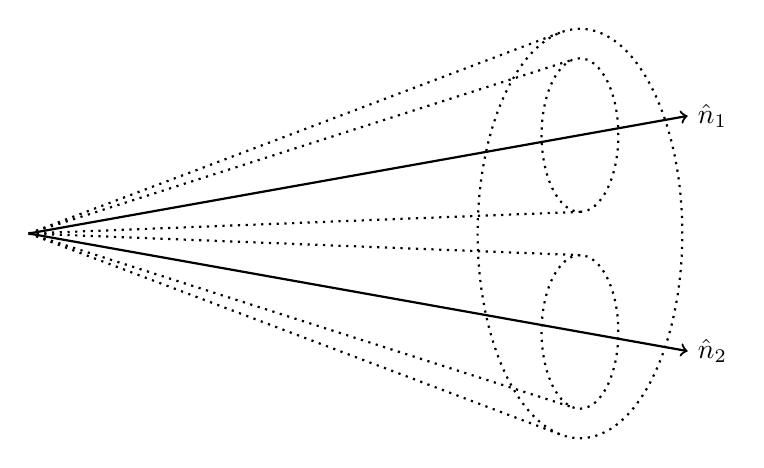
\begin{tikzpicture}
  % Main jet
  \draw[rotate around={270:(0,0)},dotted,thick] (0,7) ellipse (2.6 and 1.3);
  \draw[rotate around={270:(0,0)},dotted,thick] (0,0) -- (69.29:7.21);
  \draw[rotate around={270:(0,0)},dotted,thick] (0,0) -- (110.71:7.21);

  % Subjets
  \draw[rotate around={270:(0,0)},dotted,thick] (1.25,7) ellipse (0.975 and 0.4875);
  \draw[rotate around={270:(0,0)},dotted,thick] (0,0) -- (72.275:7.26);
  \draw[rotate around={270:(0,0)},dotted,thick] (0,0) -- (87.75:7.01);
  \draw[rotate around={270:(0,0)},dotted,thick] (-1.25,7) ellipse (0.975 and 0.4875);
  \draw[rotate around={270:(0,0)},dotted,thick] (0,0) -- (92.25:7.01);
  \draw[rotate around={270:(0,0)},dotted,thick] (0,0) -- (107.725:7.26);

  % Axes
  \draw[->,thick] (0,0) -- (10.12:8.5) node[right] {$\hat{n}_1$};
  \draw[->,thick] (0,0) -- (-10.12:8.5) node[right] {$\hat{n}_2$};
\end{tikzpicture}

  \caption{}
  \label{fig:hierarchy}
\end{figure}
